\chapter{Experiments and Evaluations}

The experiments are divided into two groups. One of which compares the extended Roofline method on memory-bound and LLC cache-bound applications using the STREAM benchmark. The STREAM benchmark is used to showcase the boundary cases. The other one uses NAS parallel benchmarks \cite{23} to compare the results on applications that are compute-bound, memory-bound and LLC cache bound. The NAS parallel benchmark suite ensures that the evaluation on the extended Roofline method covers as many types of applications as possible. 

\section{Evaluation with STREAM benchmark}
STREAM benchmark is used to evaluate the extended roofline model on memory-bound program. The problem size in STREAM source code is modified to obtain two kinds of output files namely $stream_{DRAM}$ and $stream_{L3}$. In $stream_{DRAM}$, the total memory required is much greater than the size of the L3 cache so that it can correctly measure the DRAM bandwidth. In $stream_{L3}$, the problem size is reduced so that the total memory required is less than the L3 cache but greater than the L2 cache. In this way, the STREAM is able to measure the L3 cache bandwidth correctly. The $stream_{L3}$ can be therefore characterised as an LLC-bound benchmark.

The stream benchmark and the extended Roofline method were running simultaneously on two terminal windows. The clock frequencies, PKG power, DRAM power and slowdown are recorded. Each experiment was repeated 3 times and the average value is presented. 

\begin{figure} [h] %hier können noch Positionierungswünsche angegeben werden
	\centering   % Alles weitere zentrieren
	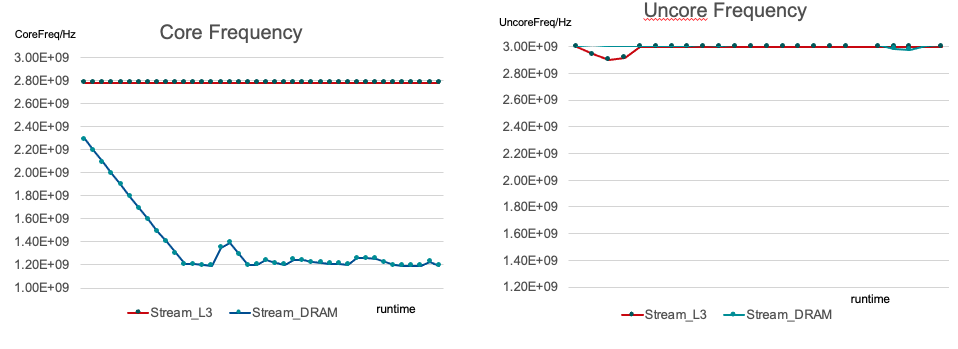
\includegraphics[width=17cm]{pictures/cuc}
	\caption{Core vs. uncore frequency of STREAM}
	%\label{fig1}  %Reihenfolge ist wichtig! Immer erst \caption{} dann \label{}
\end{figure}

Figure 5.1 illustrates the core and uncore frequency of both $stream_{DRAM}$ and $stream_{L3}$ during runtime. The x-axis shows the runtime while the y-axis represents the frequency. The figure on the left compares the core frequency of both stream programs. The core frequency of $stream_{DRAM}$ decreases linearly first and remains minimal afterwards. The reason is that the $stream_{DRAM}$ is memory intensive and it heavily utilises the memory controllers located in the uncore area. The processor core wastes large amounts of cycles stalled for memory. The extended Roofline method detects such situations and lowers the core frequency respectively. The frequency of  $stream_{L3}$ remains maximal since the extended Roofline method suggests the arithmetic intensity approximates to the machine balance. $Stream_{L3}$ is LLC intensive and most data transfers happened between L2 and LLC. The processor can access the data faster and spend less time stalling (only 1\% of the time interval). Therefore, the core frequency should not be decreased. The figure on the right shows the uncore frequency remains maximal for both stream programs because both of them utilise the uncore heavily.

	
Table 5.1 shows the PKG power in Watts, PKG energy in Joules and completion time in seconds for default setting where the core and uncore frequency is maximum. The metrics are measured with LIKWID. Figure 5.2 shows the PKG power saving and energy saving in Watts and slowdown compared to the default setting. The x-axis shows different performance groups and the y-axis represents the results that are normalised with respect to the default.

\begin{table} [h] %hier können noch Positionierungswünsche angegeben werden
	\centering      % Alles weitere zentrieren
	\begin{tabular}{|c|c|c|} %Alle Spalten zentrieren, ansonsten 'r' oder 'l'
		\hline
		\textbf{Metric} & \textbf{stream\_dram} &\textbf{stream\_L3}  \\
		\hline
		Completion time(s)              & 22 &11.5       \\
		\hline
		PKG power(W)	              &  140& 119       \\
		\hline
		PKG energy(J)		 &   2990 &   1683  \\
		
		\hline
	\end{tabular}
	\caption{Performance metrics for Stream DRAM and L3 by default when $f_c$ = 2.8 GHz and $f_{uc}$ = 3.0 GHz}
	%\label{tab:vergleich}  %Reihenfolge ist wichtig! Immer erst \caption{} dann \label{}
\end{table}

\textit{Observation 1: The extended Roofline method saves up to 40\% PKG power and energy for STREAM benchmark}

The extended Roofline method saves 38\% PKG power on $stream_{DRAM}$ compared to the default. This is because it detects the application is memory-bound and reduces the core frequency. The energy consumption also reduces due to the drop of PKG power because the energy equals the power multiplied by time. On the other hand, the extended Roofline method has minor effects on the $stream_{L3}$. The reason is that $stream_{L3}$ is balanced for computation and data communication.

\textit{Observation 2: The extended Roofline method has little impact on performance downgrading}

The job completion time is used to represent the performance downgrading. as observed from Figure 5.2, the job completion time increases by 3.2\% for $stream_{DRAM}$. This indicates the extended Roofline method has little impact on performance downgrading for memory streaming which is totally acceptable. For compute-memory-balanced programs, the performance downgrading can be ignored since the slowdown is only 0.4\%.


	
\begin{figure} [h] %hier können noch Positionierungswünsche angegeben werden
	\centering   % Alles weitere zentrieren
	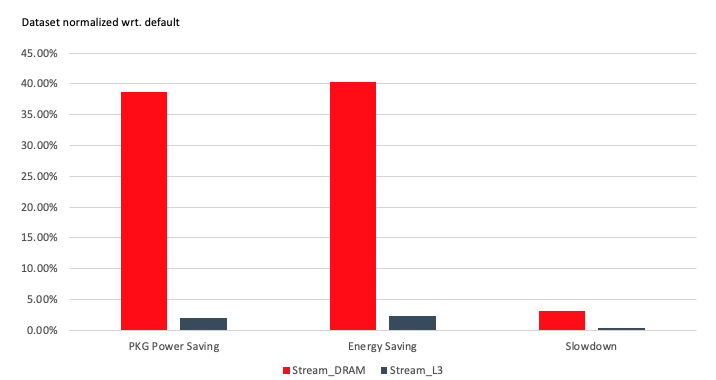
\includegraphics[width=17cm]{pictures/Stream}
	\caption{Evaluation on STREAM}
	%\label{fig1}  %Reihenfolge ist wichtig! Immer erst \caption{} dann \label{}
\end{figure}

\section{Evaluation with NAS Parallel Benchmarks}

The second group of experiments was carried out using Embarrassingly Parallel (EP),  Conjugate Gradient (CG),  Block Tri-diagonal solver (BT), Multi-Grid (MG), Fourier Transform (FT) and Scalar Penta-diagonal solver (SP) from the NAS parallel benchmark suite \cite{23}. The EP is compute-intensive, the CG is memory-bound and known for its irregular memory access and communication, MG and FT are memory-intensive programs \cite{23}. SP is LLC intensive and BT is LLC intensive with constantly changing DRAM usage \cite{21}. The openMP version of these benchmarks is used and the input sizes B and C are used in experiments.

The core and uncore frequency is maximal by default. The PKG power in Watts, PKG energy in Joules and the completion time in seconds are measured with LIKWID for the default setting. Each of the benchmarks and the extended Roofline method are executed simultaneously in two terminal windows and the performance metrics are recorded by the extended Roofline method. Each experiment is repeated three times and the average values of the results are calculated. 

Figure 5.3 presents the PKG power and energy saving and slowdown compared to the default setting. The x-axis shows the groups of those performance metrics. Each of the groups contains six columns representing EP, CG, BT, MG, FT and SP from left to right. The y-axis presents the value normalized with respect to the default measurements.

\begin{figure} [h] %hier können noch Positionierungswünsche angegeben werden
	\centering   % Alles weitere zentrieren
	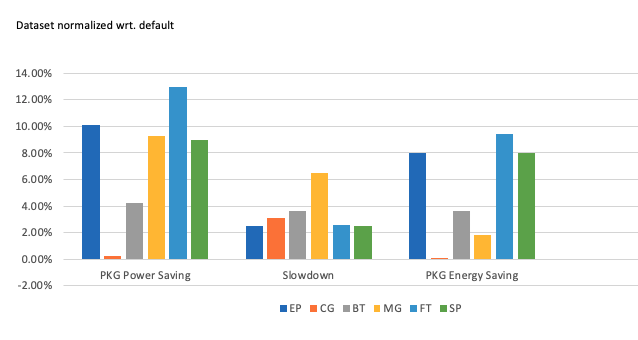
\includegraphics[width=17cm]{pictures/NPB}
	\caption{PKG power and energy saving and slowdown wrt. default}
	%\label{fig1}  %Reihenfolge ist wichtig! Immer erst \caption{} dann \label{}
\end{figure}


\textbf{EP}

The extended Roofline method achieves 10\% of PKG power saving and 8\% of PKG energy saving with a slight slowdown of 2.2\%. The program correctly detects the compute-intensive characteristic of EP. Figure 5.4 shows the activities of the CPU and memory detected by the time interval analysis. The processor occupied 83\% of the time interval while the memory is 99.8\% idle. In this case, the program sees the application as compute-bound and reduces the uncore frequency. The slowdown caused by the overhead of the program is only 2.2\% which is acceptable compared to the percentage of the power and energy saving. The slowdown on EP is one of the lowest among all other benchmarks. Therefore, the extended Roofline method performs well on compute-intensive benchmarks.

\begin{figure} [h] %hier können noch Positionierungswünsche angegeben werden
	\centering   % Alles weitere zentrieren
	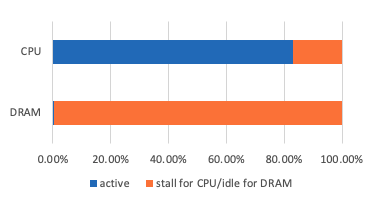
\includegraphics[width=9cm]{pictures/timeforep}
	\caption{Activities of CPU and DRAM in a sampling interval on EP}
	%\label{fig1}  %Reihenfolge ist wichtig! Immer erst \caption{} dann \label{}
\end{figure}

\textbf{CG}

The extended Roofline method has little impact on the power or energy saving on CG. It detects that CG is bound to transfer delay with memory domination. However, the core frequency is not reduced because it will lead to severe performance downgrading. As a result, the frequency should remain default for CG.  The extended Roofline method brings 3.1\% slowdown to the application because of the overhead of accessing hardware counters and interrupt for each sampling interval.

\textbf{BT and SP}

Figure 5.5 illustrates the measured core and uncore frequency. The core and uncore frequency keep being modified between 2.4 to 2.6 GHz for BT during runtime. It is because the DRAM access of BT varies during runtime. BT's execution patterns vary from memory-dominated to compute-dominated. When BT is memory-intensive, it utilises uncore heavily. The uncore frequency is higher and the core frequency is lower. When BT transits to compute-intensive, the uncore frequency becomes lower while the core frequency becomes higher. The changing of the core and uncore frequency leads to  4.2\% PKG power saving and 3.8\% of PKG energy saving. The slowdown is 3.7\% caused by standard overhead.

The extended Roofline method performs well on SP since it achieves more than 8\% of PKG power and energy saving. The slowdown is only 2.2\%. 


\begin{figure} [h] %hier können noch Positionierungswünsche angegeben werden
	\centering   % Alles weitere zentrieren
	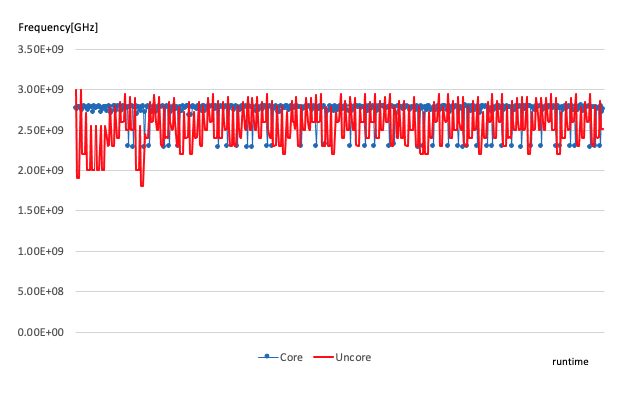
\includegraphics[width=12cm]{pictures/bt_fcuc}
	\caption{Frequency of BT from NPB}
	%\label{fig1}  %Reihenfolge ist wichtig! Immer erst \caption{} dann \label{}
\end{figure}

\textbf{MG and FT}

The core frequency is reduced and the uncore frequency remains maximal for these two memory-intensive benchmarks. The extended Roofline method achieves up to 13\% of PKG power saving and 9.4\% of energy saving. The slowdown on FT is insignificant while on MG is greater. \\

In conclusion, the extended Roofline method achieves up to 13\% PKG power saving and 9.4\% PKG energy saving with the slowdown in the worst case 6.5\%.

\subsubsection{Evaluation under the power cap}

While the frequency tuning strategy of the situations under a power cap is different from those that do not have a power cap. The evaluation of the programs under the power cap is also needed. In this experiment, RAPL is used to set the power cap of the processor. The power cap is set to the minimum which is 69W to compare the extended Roofline method with the default setting. Figure 5.6 shows the total energy saving (PKG + DRAM energy) and the speedup with respect to the default on the NAS parallel benchmark suite under the power cap. The x-axis shows the groups of the performance metrics. The y-axis presents the data normalized with respect to default. The extended Roofline method achieves up to 6.2\% speedup over default. It reveals that the extended Roofline method outperforms the default setting under strict power constraints. Spending less time completing the tasks leads to less energy consumption. During the experiment, the extended Roofline method keeps the power consumption lower than the default. Lower power consumption and shorter execution time lead to 8.9\% energy saving in the best case across all benchmarks

\begin{figure} [h] %hier können noch Positionierungswünsche angegeben werden
	\centering   % Alles weitere zentrieren
	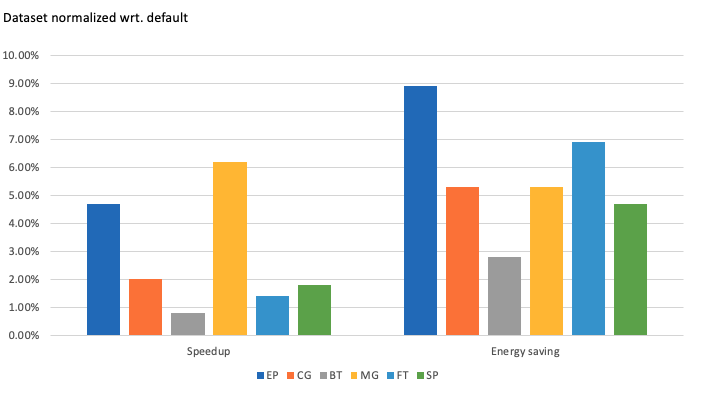
\includegraphics[width=15cm]{pictures/cap}
	\caption{Total energy saving and speedup wrt. default under power cap}
	%\label{fig1}  %Reihenfolge ist wichtig! Immer erst \caption{} dann \label{}
\end{figure}





